\section{Fertige Landingpage [L]}
Die Landingpage (siehe Abbildung \ref{fig:impl:finishedLandingpage}) repräsentiert das Projekt, denn es ist das erste, was ein neuer Benutzer*in von der Webanwendung zu sehen bekommt. Es war wichtig, ein modernes Design dafür zu entwickeln.

Wichtige Punkte, die bei der Landingpage beachtet wurden, waren die Hierarchie der Elemente. Zuerst gab es eine Einleitung, um das Projekt zu erklären, danach kam ein großer Knopf, der dazu einlädt, das Produkt zu verwenden. Er verlinkt zu der Anmeldung. Danach kam eine Selektion aus den neuesten erstellten Ausstellungen, damit kann sich der User gleich ein Bild vom Projekt machen.

\begin{figure}
    \centering
    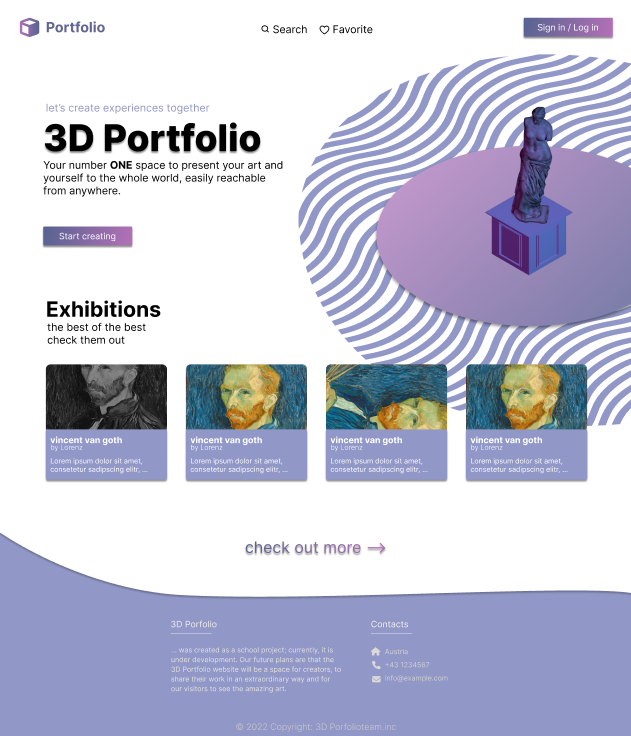
\includegraphics[scale=.5]{pics/startingpage.png}
    \caption{Landing Page}
    \label{fig:impl:finishedLandingpage}
\end{figure}

Um zwischen den verschiedenen Unterseiten der Webseite zu wechseln, wurde am oberen Bildschirmrand zusätzlich eine Navigationsleiste implementiert. Diese sogenannte Navbar besitzt je nach Unterseite verschiedene Designs. Dies ermöglicht ein angenehmes Navigieren auf jeder Seite (Siehe Routing \ref{lst:impl:routing}). Ebenfalls muss auch der Footer auf jeder Unterseite passend angezeigt werden. Um das Design der Navbar und Footer auf jeder Seite individuell zu gestalten, wird ein Service jeweils in die entsprechende Komponente injiziert. Dadurch können Konfigurationen am Design durch wenig Code und Redundanz vorgenommen werden. 

\subsection{Erledigte Userstories [L]}
Bei der Fertigstellung der Landingpage wurden folgende Userstories vollendet: 
\begin{compactitem}
    \item Als erstmalige*r Besucher*in der Webseite möchte ich die benötigten Informationen über die Funktionen der Applikation verständlich erkennen können. Akzeptanzkriterien:
    Auf der Landingpage befinden sich:
    \begin{compactitem}
        \item Textstellen und Grafiken, die unser Projekt und die Funktionalitäten davon erklären
        \item Einen Call-to-Action(CTA)-Button, der den User*in dazu einlädt, seine eigene Ausstellung zu erstellen. Beim Betätigen wird der Benutzer, falls er schon eingeloggt ist, weitergeleitet zum Editor, sonst zur Login Seite (hier gibt es die Möglichkeit, sich auch einen Account zu erstellen)
    \end{compactitem}
\end{compactitem}

